\chapter{Strumenti e tecnologie}
\label{chap:strumenti}

In questa sezione vengono introdotti gli strumenti e le tecnologie utilizzate per lo sviluppo della \textit{Web Application}. La scelta di questi si è basata principalmente sulle conoscenze e sull'esperienza del team di sviluppo. 

\section{Spring}

\begin{figure}
\begin{center}

\includegraphics[width=0.5\columnwidth]{images/springlogo.png}
\end{center}
\caption{Logo Spring Framework}
\label{fig:springf}
\end{figure}

Per il \textit{back-end} è stato scelto Spring, che è un \gls{framework} molto utilizzato e supportato per le
moderne applicazioni basate su Java. Il lavoro principale svolto da Spring è la semplificazione dell'unione e dei collegamenti delle parti dell'applicazione, permettendo agli sviluppatori di concentrarsi unicamente sulla logica di business. È basato su
concetti chiave come l’\textit{inversion of control} e la \textit{dependency injection} \cite{spring}.\\

L'\textit{inversion of control} è un pattern per cui un componente di livello applicativo riceve il controllo da un componente appartenente a un libreria. Lo scopo di questo pattern è quello di rendere le parti del sistema software più indipendenti fra loro, ottenendo così la possibilità di effettuare modifiche senza coinvolgere altre parti del sistema \cite{ioc} \cite{baeldung}. \\

La \textit{dependency injection} è il secondo concetto chiave, attraverso questo \gls{designpattern} è possibile implementare l'\textit{inversion of control}. È una tecnica in cui un oggetto acquisisce le dipendenze necessarie in fase di creazione, quando gli viene \textit{iniettato} un oggetto,
il quale viene poi utilizzato come servizio dall’oggetto principale \cite{depinj} \cite{baeldung}.



\subsection{Spring Boot}
\begin{figure}
\begin{center}

\includegraphics[width=0.8\columnwidth]{images/springbootlogo.jpg}
\end{center}
\caption{Logo Spring Boot}
\label{fig:springboot}
\end{figure}

Spring Boot è una soluzione \textit{"convention over configuration"} riduce la complessità di configurazione di nuovi progetti Spring. A questo scopo, Spring Boot definisce una configurazione di base che include le linee guida per l'uso del \gls{framework} e tutte le librerie di terze parti rilevanti, rendendo quindi l'avvio di nuovi progetti il più semplice possibile \cite{springboot}.


\subsection{Spring Data}
\begin{figure}
\begin{center}
\includegraphics[width=0.3\columnwidth]{images/springdata.png}
\end{center}
\caption{Logo Spring Data}
\label{fig:springdata}
\end{figure}
Spring Data ha lo scopo di fornire un modello di programmazione per l'accesso ai dati e per la gestione della persistenza di essi. Definisce un’insieme di \gls{API} per semplificare l'utilizzo di tecnologie che si interfacciano con database relazionali e non. Questo progetto contiene molti sottoprogetti specifici di un determinato database. In particolare nella \textit{Web Application } è stato utilizzato Spring Data JPA che 
fornisce l’accesso a database relazionali e ne permette la gestione tramite oggetti Java.
Il \gls{DBMS} utilizzato è stato Oracle e tramite questo modello è stato possibile mappare le tabelle del database con oggetti \cite{springdata}.

\clearpage

\subsection{Spring Security}

\begin{figure}
\begin{center}

\includegraphics[width=0.45\columnwidth]{images/springsec.jpeg}
\end{center}
\caption{Logo Spring Security}
\label{fig:springsec}
\end{figure}

Spring Security è un \gls{framework} di autenticazione e controllo degli accessi altamente personalizzabile. È lo standard \textit{de facto} per la protezione delle applicazioni basate su Spring. Per garantire l'accesso alla \textit{Web Application} ai soli utenti autorizzati si è utilizzato inoltre il meccanismo di autenticazione \textit{JWT}. Questo meccanismo è diventato uno standard che viene usato per “regolare” le richieste tra  \textit{client} e \textit{server}. Dopo l'esito positivo dell'autenticazione il server genera un \textit{token}, ovvero una stringa \textit{JWT}, contente informazioni specifiche per l'utente, tra cui anche la scadenza del \textit{token}. Ad ogni successiva richiesta da parte del \textit{client} di accedere a determinate risorse del \textit{server}, verrà richiesto il \textit{token} e avverrà il controllo di esso. Di seguito uno schema riassuntivo del meccanismo :

\begin{figure}
\begin{center}
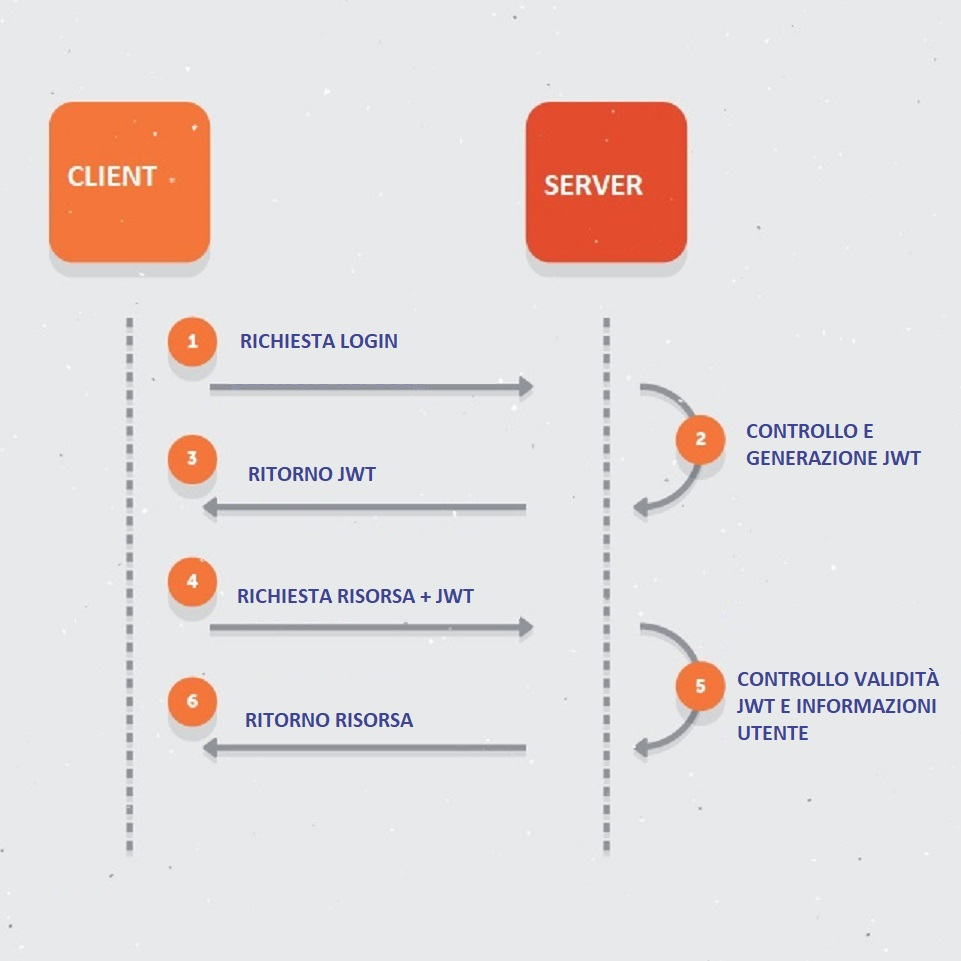
\includegraphics[width=0.6\columnwidth]{images/jwt.jpg}
\end{center}
\caption{Schema riassuntivo meccanismo JWT}
\label{fig:jwt}
\end{figure}



%\foreignlanguage{english}{\Blindtext}

\section{Angular}

\begin{figure}
\begin{center}

\includegraphics[width=0.17\columnwidth]{images/angularlogopng.png}
\end{center}
\caption{Logo Angular}
\label{fig:angular}
\end{figure}

Angular è un \gls{framework} molto utilizzato per lo sviluppo di applicazioni web, in particolar modo della parte riguardante il \textit{front-end}. Sviluppato principalmente da Google, è l'evoluzione del suo predecessore AngulaJS, le due versioni non sono compatibili. Il linguaggio di programmazione usato per la prima versione è JavaScript mentre quello di Angular è TypeScript. Quest'ultimo, è un linguaggio di programmazione sviluppato da Microsoft \cite{angular}.
Nasce dal crescente bisogno di un linguaggio \textit{front-end} per lo sviluppo di applicazioni JavaScript su larga scala e dalla necessità di sicurezza e robustezza.
Il linguaggio estende la sintassi di JavaScript in modo che qualunque programma scritto in JavaScript sia anche in grado di funzionare con TypeScript senza nessuna modifica. È destinato a essere compilato in JavaScript per poter essere interpretato da qualunque web browser \cite{typescript}. I costrutti principali di questo framework sono: \cite{angulararchi}
\begin{itemize}
    \item \textit{Component}: è l’elemento principale di un’applicazione Angular.
    Esso contiene la logica di interazione dati e utente che definisce l’aspetto ed il comportamento della vista. Un \textit{component} quindi è un singolo elemento dell'interfaccia utente, dotato di caratteristiche univoche e che è possibile collegare chiaramente ad altri elementi dell'interfaccia \cite{component}.
    \item \textit{Service}:  è una classe che viene definita per svolgere un compito ben preciso ed effettuare delle operazioni strettamente correlate tenendo in mente il principio di singola responsabilità. Esempi di questi compiti sono: reperimento dei dati dal \textit{server}, gestione degli errori e scambio di dati tra \textit{component} \cite{service}. 
\end{itemize}

\subsection{Bootstrap}

\begin{figure}
\begin{center}

\includegraphics[width=0.11\columnwidth]{images/bootstraplogo.png}
\end{center}
\caption{Logo Bootstrap}
\label{fig:bootstrap}
\end{figure}

Per rendere l'interfaccia grafica più \textit{user-friendly} si è utilizzato Bootstrap, una raccolta di strumenti basati su HTML, CSS e JavaScript che fornisce componenti già formattati e visualmente
piacevoli come bottoni, barre di navigazione, \textit{card} e molti altri.








